\chapter{Programme}
\section{Team Structure}
The Programme team was comprised of Anya Sier and Nuala O'Rourke as the Programme Coordinators, with a lot of support from Millie Burgh, Woodcraft Folk Events Assistant. Millie did most of the work until May 2023 due to Anya and Nuala having other educational commitments. Nuala found out she was unable to attend camp and disengaged. \\

Millie took the lead on booking the evening programme performers, recruiting centre coordinators and volunteers as well as planning the adventurous activities with the Biblins' Activities Coordinator. She also worked out a structure for the programme and mini-themes. Anya took the lead on coordinating four centres (Activism, Arts, Mythology and MEST-UP) with the remaining (Radio, Media and Cinema) self-coordinating. Anya also worked with another volunteer to coordinate the Wide Game.
\subsection{Evaluation of Team Structure \& Support}
While the team structure worked, it put a lot of pressure on a very small team to make Programme happen. Ideally, you need at least two people to coordinate the programme as their full time role, with these two continuing onto site to manage programme delivery. You should also have two coordinators for each centre. 

The team found that there was a drop in capacity during Anya's exam period, which whilst expected, hadn't been planned for causing issues. They should have worked out what could have been done earlier and drafted in additional support. \\

There was a lot that needed to be done in the final few months, which Anya managed, with some limited support from Millie who was also juggling other tasks for the camp. This was Anya's first time in a central role like this, and she was unsure who to reach out to. Support increased as camp approached, however earlier guidance would've been appreciated. Anya suggested that having an `understudy' would be a good idea, as it would allow a Venturer or DF to be trained up and feel more confident doing this role.


\section{Supporting Events}
\subsection{Pre-Camp}
Only 1 person made it to the Programme Online Pre-Camp session. They found that the Q\&A element was the most useful part of it. It was suggested that the session could be targeted more towards Venturers, given that it was programme based and they would be encouraged to engage with it. \\

No one from the Programme team was able to make it to On-Site Pre-Camp. It was also noted that the aims of the weekend hadn't been made clear and that may have improved attendance. 
\subsection{Working Week}
Anya was able to make it to working week which she found vital to the success of the role. She was able to divide up supplies, ensure the right tents were put up and sort furniture for centres. She had planned to make a start on getting centres setup, however was unable to get very far due to running out of time. She noted that MEST-UP needs someone to attend Working Week, especially since they have to also set up the Safe Space. If the coordinator can't make it in the future, then another volunteer from the MEST-UP team should be sent. 

\section{On-Camp Operations}
\subsection{Daily Structure}
Anya had a very busy time on camp, exasperated by the fact that she was working on her own in the role of Programme Coordinator. Her mornings involved preparing and circulating the day's programme. This calmed down towards the end of the camp, enabling her to have some time off. Afternoons involved overseeing the workshops to ensure they were full and making good progress, as well as ensuring that the Centre Coordinators were able to get a break and dinner. The evenings were filled with supervising the progress of evening activities, however this was a challenge as Anya also had leadership commitments within her own group. 
\subsection{Support}
Anya managed to get time off here and there throughout the week and take a full day off. The programme team felt well supported by the Volunteer Support Team. The programme team also gained support from the coordinator, although this was lacking until the Programme Coordinator was close to breaking point. The Centre Coordinators provided a good and supportive team, however it felt like there was more support for the core team than the members of the wider team. Despite this, the Centre Coordinators did feel supported - with the programme coordinator taking the brunt of the stress. The centre coordinators suggested to make PEB more accessible and known to a wider audience.

\section{Programming Specific Insights}
\subsection{Programme Issues On Camp}
As would be expected, there were a number of issues with the Programme. The primary issue being related to permissions for Sex Education Workshops within the MEST-UP centre. We required every participant to have consent to be able to take part in SRE (Sex \& Relationships Education) beyond the initial consent workshop which was a compulsory part of the camp programme. A number of campers didn't have this consent, and as such they could not be permitted to take part in MEST-UP workshops around Sex \& Relationships. For future events, the Safeguarding team needs to support in advance of the event with working out what content we can deliver and where the boundaries should be. MEST-UP need to be involved in the conversation, to ensure that the boundaries are realistic for them to be able to deliver to.\\

Challenges were also experienced with external facilitators activities' due to the lack of promotion and engagement. A number of facilitators were brought onto site to run sessions which had very low engagement. For future events - it's recommended to advertise these sessions more through the news \& providing printed programmes. It would also be worth running consultation with Venturers to understand what types of workshops they want to see from external organisations.\\

The concept of Mini-Themes, where a few days would have a sub-theme relating to Mythology, also didn't work very well. This could be due to centres not implementing this into their programme, perhaps due to not being told far enough in advance, but it could have also been due to lack of advertising of the Mini-Themes. It would have helped to have a Programme Guide which explained this in more detail than what we released.

\subsection{Miscellaneous Insights}
There were additional challenges with using Biblins as a site for Venturer Camp, including the site not being truly accessible and the lack of signal across the site. This was especially a challenge while attempting to coordinate with External Organisations or Bands.\\

It helps for the programme team to have bikes available, so they can get between the different bits of the site easier \& quicker. It also felt useful to have the centre coordinators and programme coordinator in the same village, as this allowed for easy communication. \\

For future events, the Programme Coordinator suggests not to get too stressed about issues arising throughout the camp, promoting externally facilitated sessions and to make announcements after the news about that evening's programme \& the big sessions on the subsequent days. \\

The Cinema Tent required a Umbrella License from the Motion Pictures Licencing Company Limited. This is valid for one year for the organisation, and costs approximately £150. This license is required to be able to display films and other media live.

\subsection{Daytime Programme}
The centres which operated in the daytime were as follows:
\begin{itemize}
    \item Activism - Coordinated by Cherry Tucker
    \item Mythology - Coordinated by Tom Egan-Payne, Dermot O'Rourke and Colm Andrews
    \item Arts - Coordinated by Carmen Mallinson-Pocock
    \item MEST-UP - Coordinated by Isla Douglas with the DF MEST-UP Team
    \item Media - Coordinated by Gus Canham
    \item Radio - Coordinated by Tyler Eckersall
    \item Cinema - Coordinated by Ash Taylor
\end{itemize}

% Map here

The layout generally worked well. The programme coordinator said it was weird having the footpath at the back of the central area as it made it a bit difficult to get people in without a clear `through path' and lots of public on the footpath.\\

\begin{figure}[ht]
    \centering
    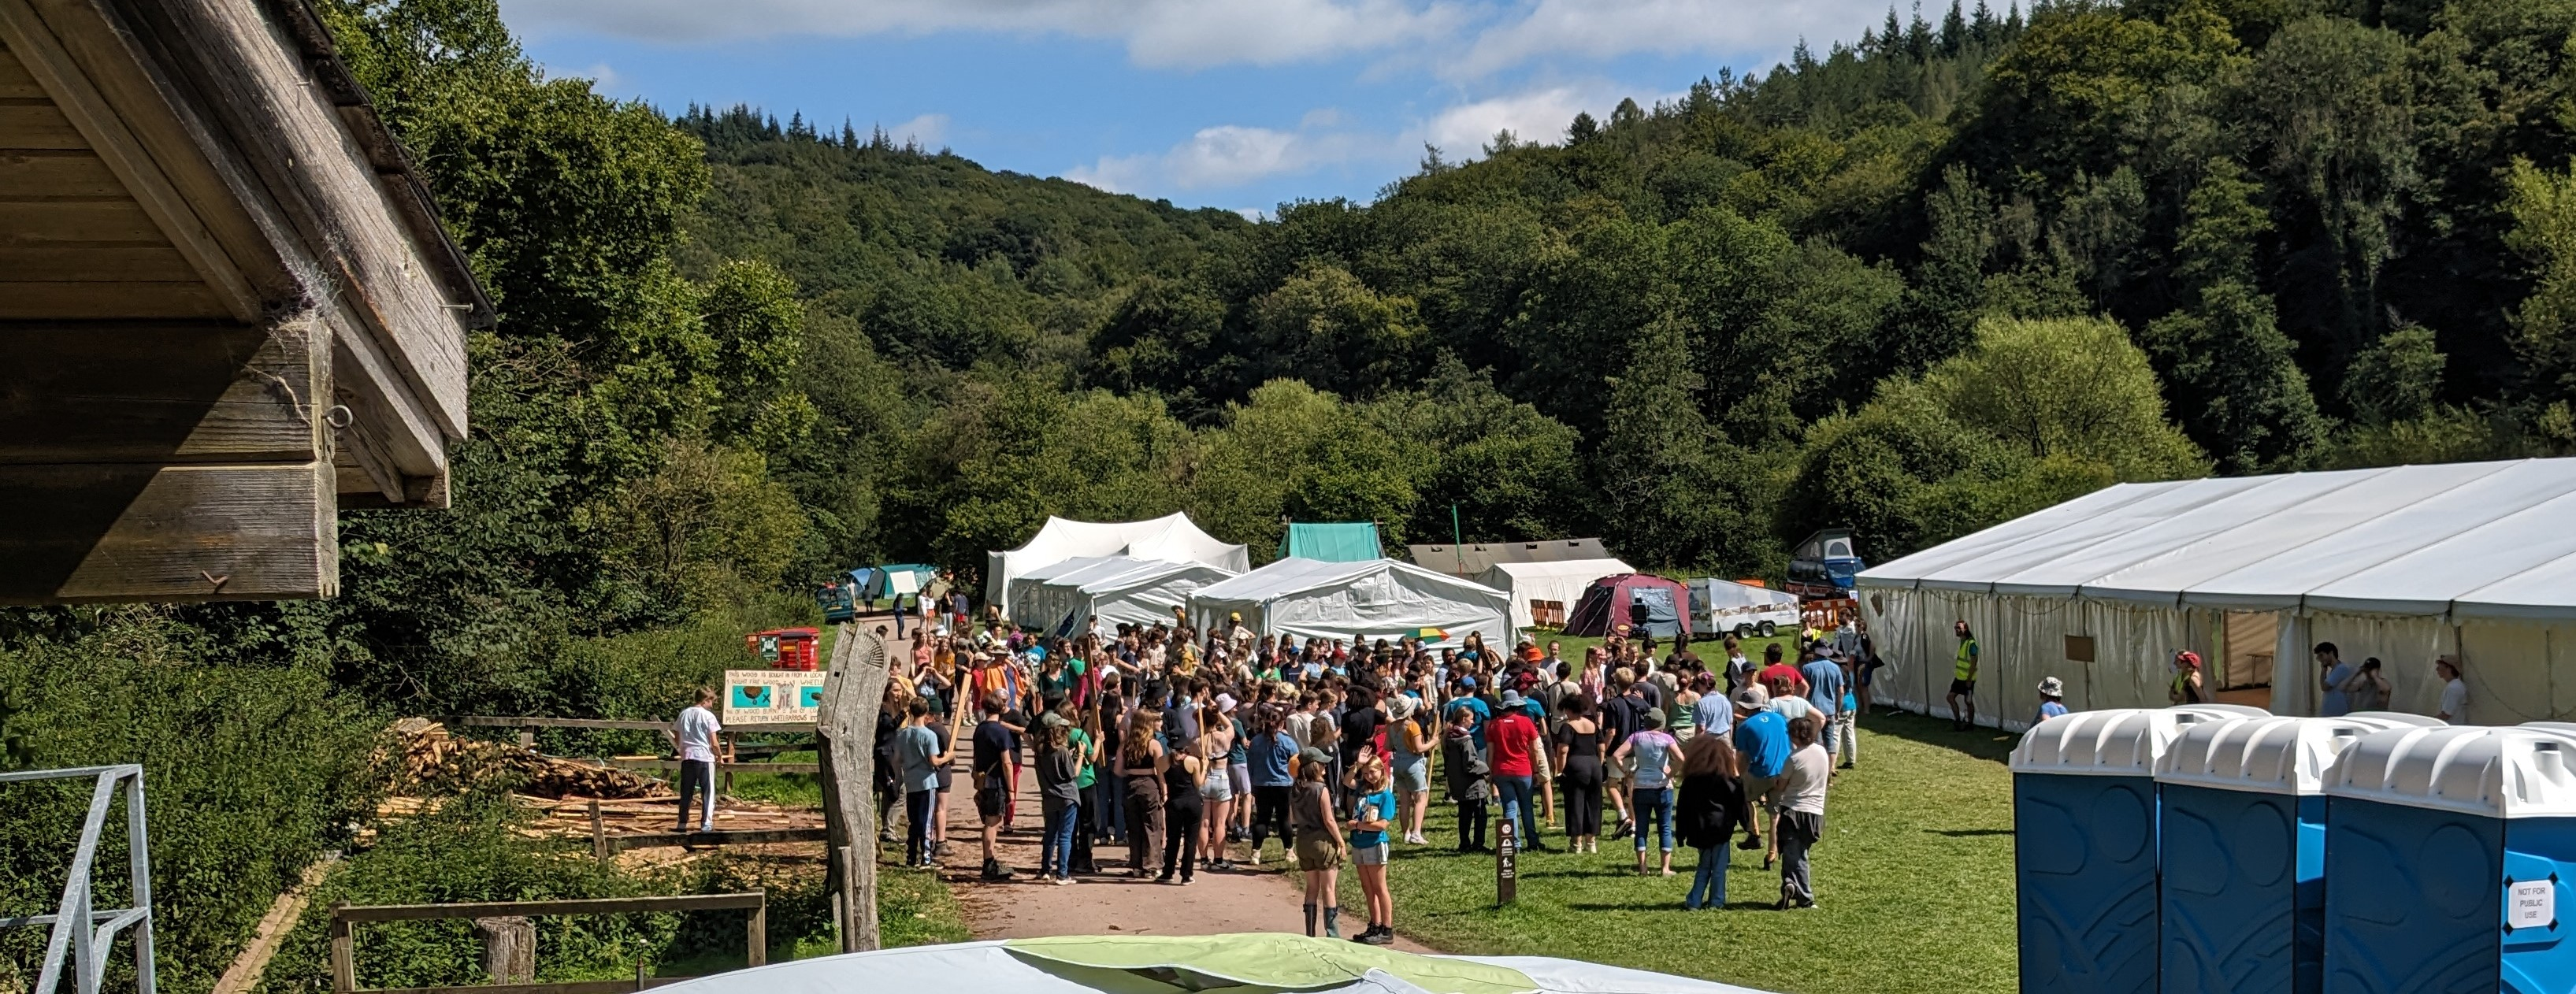
\includegraphics[width=0.8\textwidth]{assets/wide-game-battle.jpg}
    \caption{Final battle at the end of the Wide Game (\textit{TB})}
\end{figure}

Within the central area it was lovely but very close to the footpath. It's perhaps not the best to have radio and cinema next to each other due to noise. Something that isn't clear on the map is that MEST-UP had a workshop/drop in tent and a separate tent as a safe space.
\subsubsection{Equipment}
It worked well doing a bulk order for stationary from YPO and asking centre coordinators what they needed to add to this. It also worked well to allocate each centre the size / kind of tent, the number of tables and chairs and the amount of power that we thought they needed and tell them rather than ask them what they wanted as often it's a lot of work negotiating this with what equipment / power we have available. There didn't seem to be any complaints about this. Centres got their own budget for anything else they needed e.g decoration, specific resources not available on YPO or expensing guest workshop facilitators but many didn't use much of this if any. Some centres requested floor coverings, in the form of tarps as they would be sitting on the floor. We were able to scavenge some for this, however it would be beneficial to source these further in advance in the future.
\subsubsection{Adventurous Activities}
Ahead of camp, the Events Assistant organised canoeing and climbing with Alex, the Activities Coordinator at Biblins. The idea was that every participant should get the chance to do at least one of these should they wish to. We booked for two morning sessions and one afternoon session of both canoeing and climbing, on the Monday, Tuesday, Thursday and Friday of camp. This should have enabled 144 venturers to canoe, and 144 venturers to climb, which we predicted would be enough. The plan was that each village would get a day to offer their venturers these sessions and we would hand out a sign up sheet at the village coordinator meeting the morning before so they could plan who would do what. In the end the two smallest villages shared a day because bookings went up and we created a fifth village. We didn't want to run these sessions on the first full day as everyone needed to be at the consent workshop and we wanted to give everyone a chance to explore and get to know the centres and site. And we didn't want to run them on the Wednesday because we wanted everyone to be involved in the wide game. The bulk of the cost for this comes from hiring the canoes, and that makes it difficult to have more than 12 young people canoe at once. But Biblins are hoping to purchase some soon and this would make it a lot cheaper and therefore a lot easier to run as an activity.\\

The canoeing plan had to be changed at the start of camp because there was uncharacteristically high rainfall and as a consequence the river was flowing too fast to do static sessions. We worked with Mike to come up with the best way to still give as many venturers the chance to canoe as possible. The solution was to offer sessions where participants canoed down the river. This meant we could  only offer one canoeing session in the morning rather than two, and we had to ask groups to help pick up / drop off young people where they would end or start the sessions in minibuses and cars they had on site. It was a struggle offering everyone an adventurous activity session with this revised plan, but in the end due to the river slowing down and Mike offering his time we were able to offer an extra session on the Friday, so very few young people missed out.\\

In the future it may be worth planning for the worst in terms of weather and then we can offer more sessions if possible, to avoid the stress of last minute changes on both the central team and group leaders.\\

The Programme Coordinator wasn't really involved in any of the discussions around these activities, which made her feel a bit isolated. She was asked questions about them but didn't know what was going on.

\begin{figure}[ht]
    \centering
    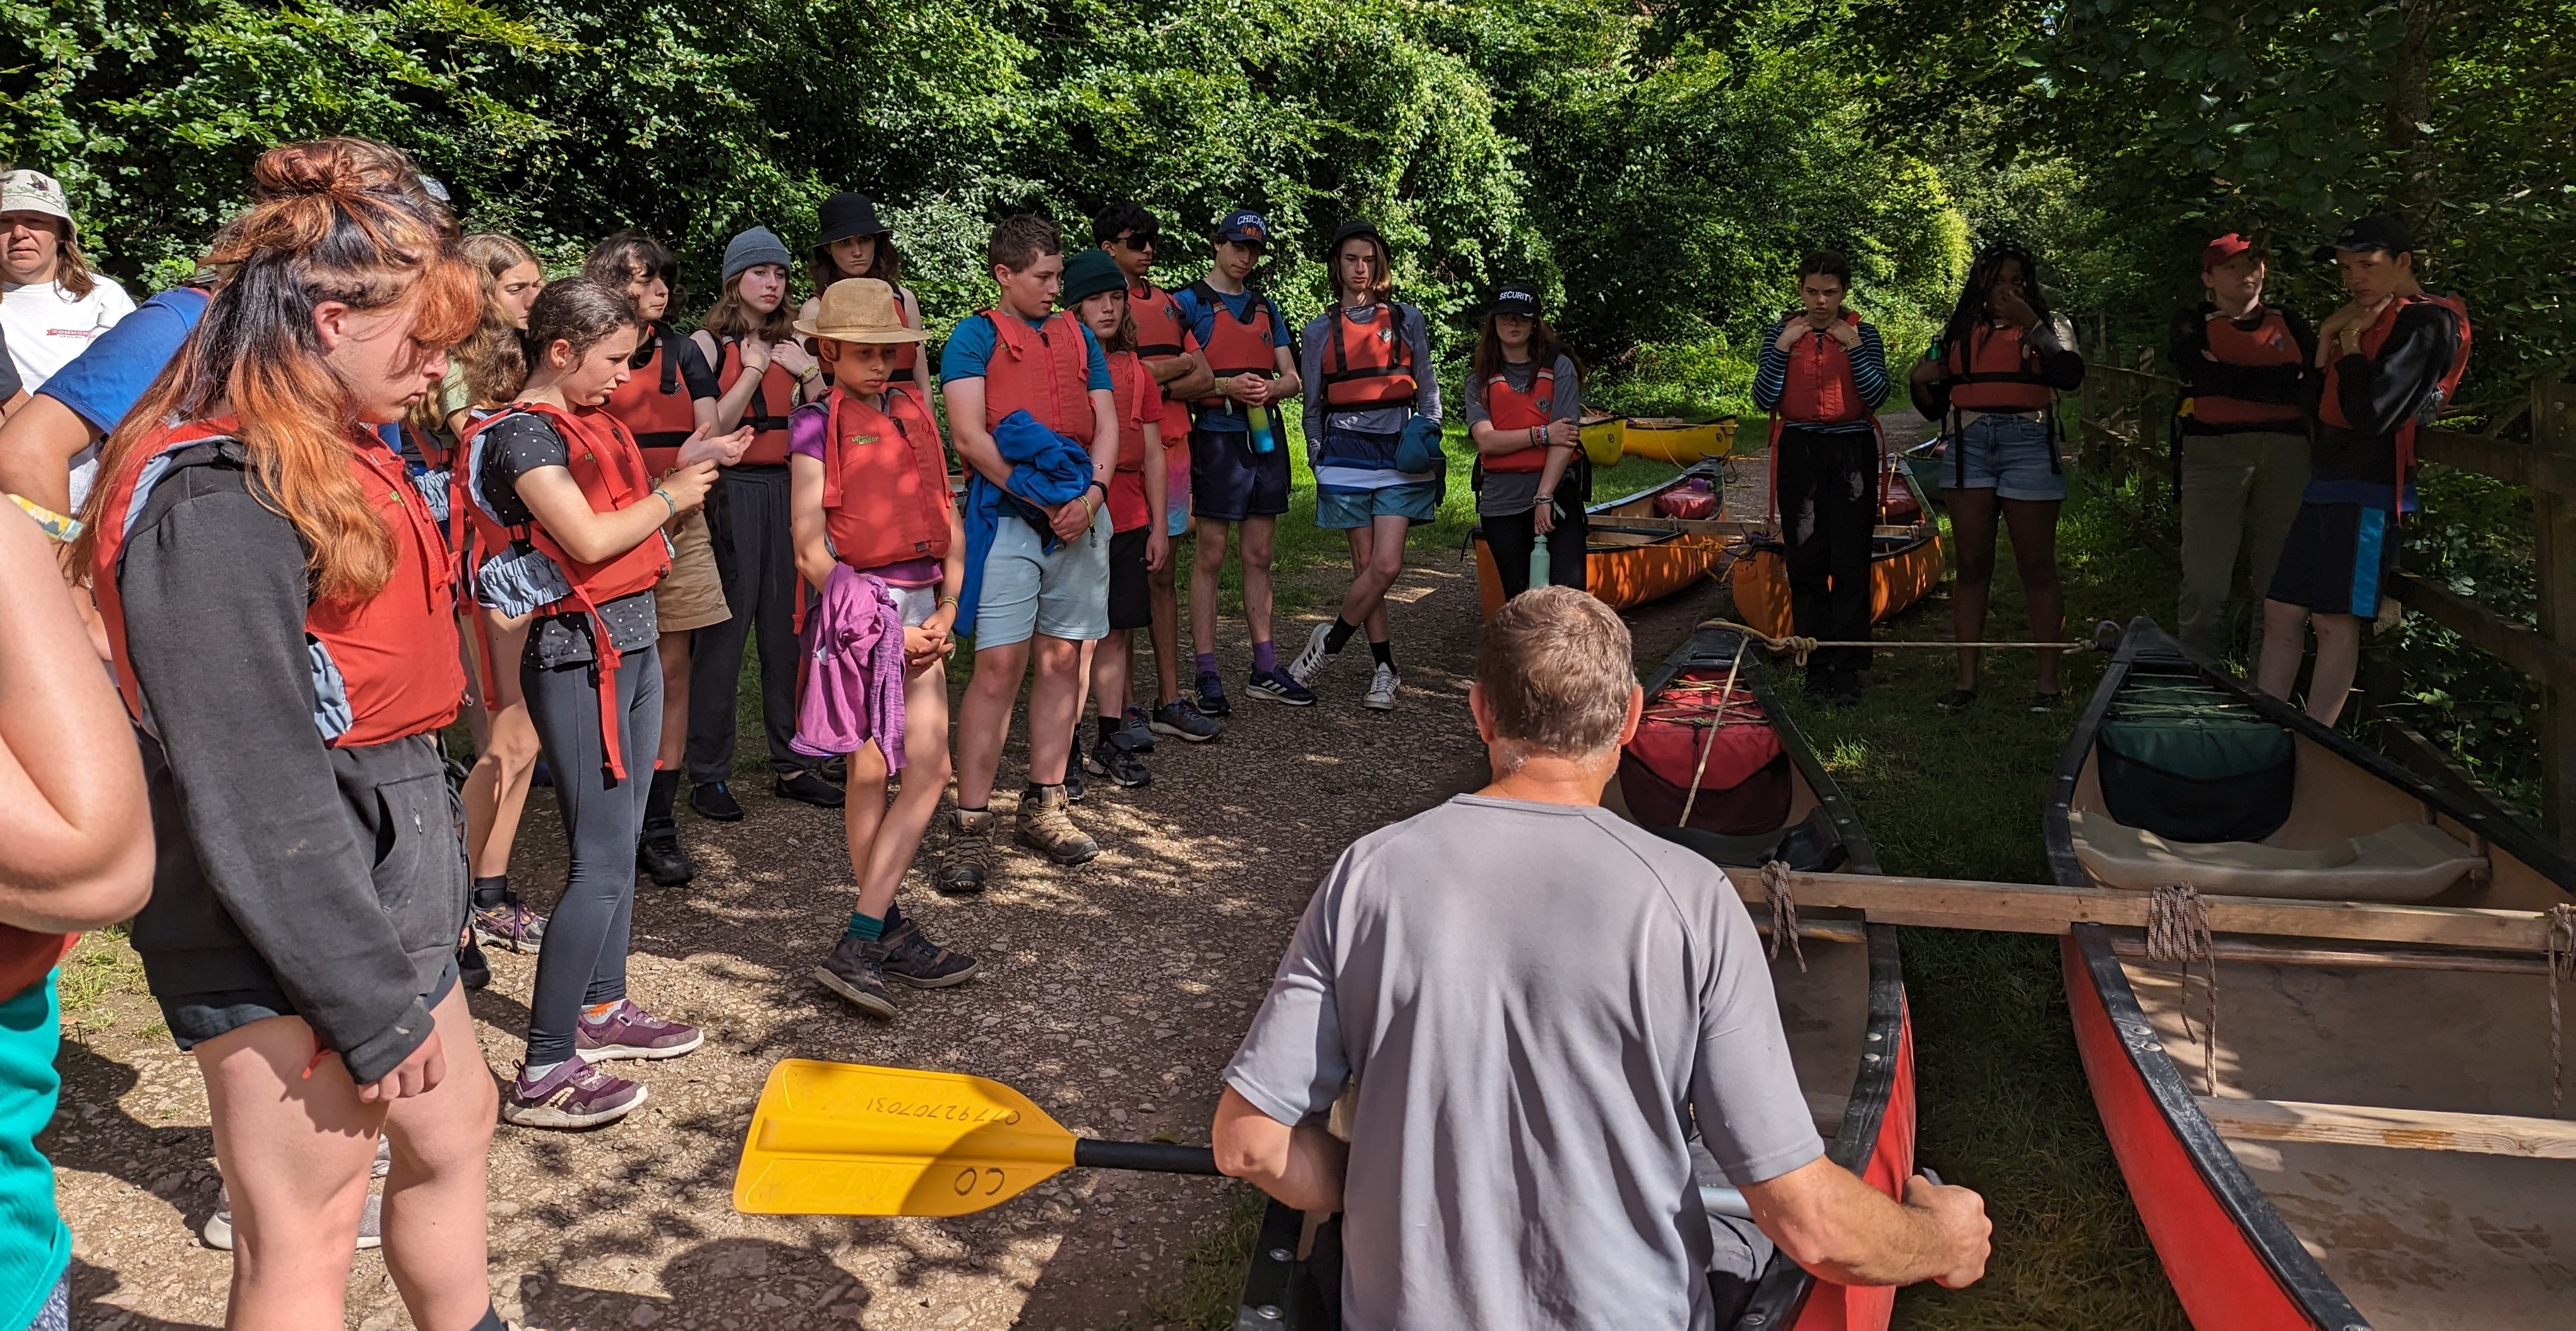
\includegraphics[width=0.8\textwidth]{assets/adventurous-activities-rs.jpg}
    \caption{Canoeing group preparing to launch (\textit{RS})}
\end{figure}
\subsection{Evening Programme}
The timescale of planning and budget for this camp made it difficult to get any big name performers in unfortunately. The Events Assistant used a spreadsheet provided by the Evening Programme Coordinator from Common Ground to ascertain some local performers worth contacting (luckily they lived in Bristol so most of the performers were based in the West Country). The Events Assistant also asked for input from Venturers on the socials. We knew we definitely wanted a Merry Moot one night which wouldn't require booking anyone. We also wanted a ceilidh one night so we looked into ceilidh bands from past events, but unfortunately these were all too busy or expensive so we went with someone the Head of Centres knew in Wales.\\

It was decided we should have an evening programme every other night as it is usually the case to have some chill nights, and we wanted a variety of music the two nights remaining. The Events Assistant contacted many performers but the majority never responded and a few were unavailable. Below are all the performers we booked / seriously considered, the ones that we had in the end in green.\\

In the spring we were worried about finances, so we decided to not book any more performers that cost money. We did a callout for budding DJs and a couple responded but no one really had time to sort this on camp so they weren't able to play until the last night. It would be worth calling on these two in future now they know the ropes though. As they are under age 18 as of releasing this report - please contact Venturer Camp 2023 Coordinator, Thomas Boxall, for their names and contact information. 

\begin{figure}[ht]
    \centering
    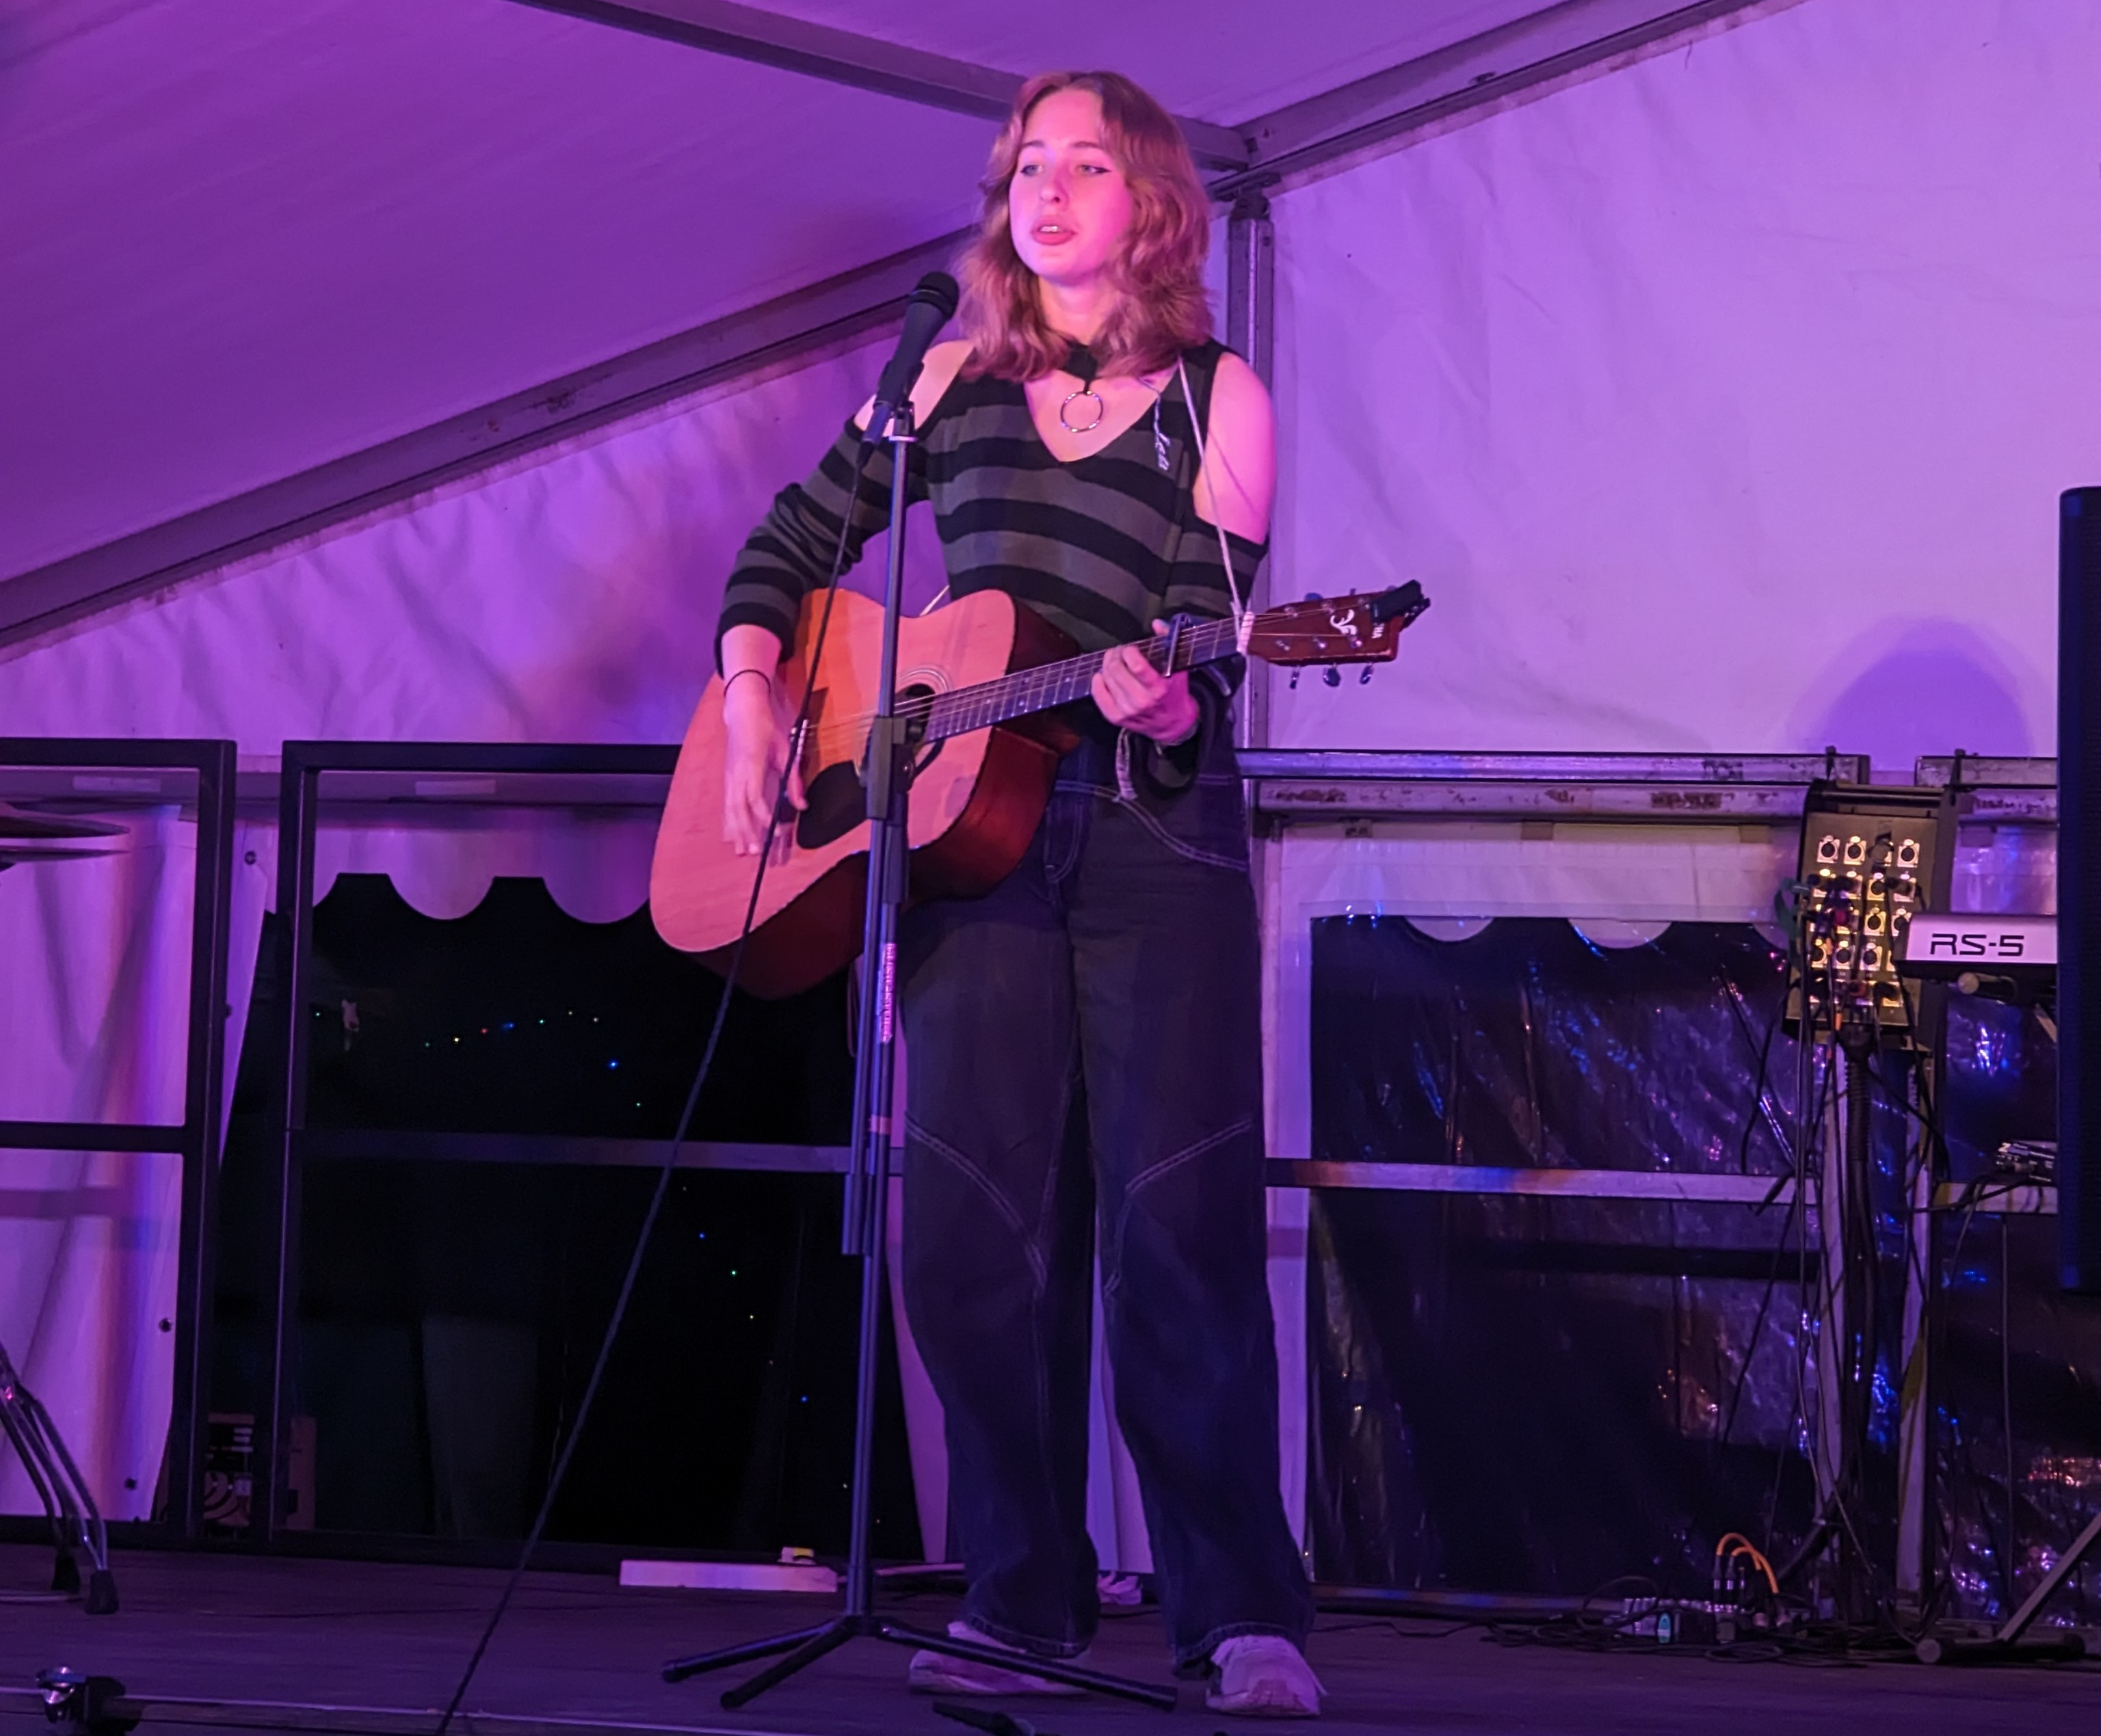
\includegraphics[width=0.8\textwidth]{assets/evening-performance-rs.jpg}
    \caption{Performer at the Merry Moot (\textit{RS})}
\end{figure}

{\RaggedRight \centering
\begin{longtable}{p{0.2\textwidth} p{0.2\textwidth} p{0.1\textwidth} p{0.1\textwidth} p{0.3\textwidth}}
\textbf{Band / Performer} & \textbf{Date / Time} & \textbf{Style} & \textbf{Fee (if booked)} & \textbf{Other Info} \\ 
\hline
\endhead

\multicolumn{5}{r}{\footnotesize\itshape continued on next page}\\
\endfoot 

\endlastfoot

\rowcolor[HTML]{EA9999} 
Spitfire Tides & Sat 5, 8:30 - 10? & Indie Rock - a lot like the arctic monkeys & Quoted 200 & We decided against them and they were no longer available once SBB cancelled \\
\hline
\rowcolor[HTML]{F9CB9C} 
Sunshine Blues Band & Sat 5, 9 - 10 & Blues & Quoted 200 & Band split up and cancelled on us. Only discovered this emailing for tech reqs 6 weeks before camp! \\
\hline
\rowcolor[HTML]{B6D7A8} 
Bunny Eye Ceilidh & Mon 7, 8:30 - 11:30 & Celtic folk (with ceilidh caller) & 550 & Not recommended. Dances at the start weren't great and the caller was rude to Scottish venturers \\
\hline
\rowcolor[HTML]{B6D7A8} 
Luna & Weds 9, all night to host Merry Moot with a couple of her own numbers & Venturer drag queen, pop music esp Abba! & Free! & Recommended. Excellent performer and free! also hosted an Abba party on the first night when we were unable to replace cancelled band \\
\hline
\rowcolor[HTML]{B6D7A8} 
Hunny Buzz & Fri 11, 8:30 - 10 & Indie Rock & 350 & Recommended. Very popular with venturers and gave us a discount \\
\hline
\rowcolor[HTML]{B6D7A8} 
Jonny Helm and Carmen M-P & Fri 11, 10:30-11 & Fire performers & Free! & Recommended. Excellent performers, free and good to have something different esp for opening or closing! We organised on site, but if you do a callout in advance more people could bring equipment (lots of fire performers in WCF) \\
\hline
\multicolumn{3}{r}{\textbf{Total}} & 900 & \\
\hline
\multicolumn{3}{r}{\textit{Left In Budget}} & 850 & \\
\hline

\caption{Evening Programme Options at Venturer Camp 2023}
\end{longtable}
}% end of \RaggedRight

\subsection{Timeline}
\subsubsection{Autumn}
\begin{itemize}
    \item Theme chosen. 
    \item Key decisions made about the programme over the week (e.g when are centres open? When is the wide game? When is the evening programme?)
    \item Programme coordinators recruited. 
    \item Centre themes decided. 
    \item Begin recruiting centre coordinators. 
\end{itemize}
\subsubsection{Winter}
\begin{itemize}
    \item Performances / workshops booked with anyone we want to prioritise / are really keen to get.
    \item Daily / weekly itinerary planned with timings.
\end{itemize}

\subsubsection{Spring}
\begin{itemize}
    \item Centre coordinators all recruited. Recruit centre helpers.
    \item Booked in everyone else we want for the evening programme, fill in gaps by calling out to Members on social media to DJ / perform.
    \item Working with Comms people to get programme info on social media, in info packs etc
\end{itemize}
\subsubsection{May}
\begin{itemize}
    \item Pre-Camp prep.
    \item Wide game planning with another volunteer.
    \item Consult centres on where they want to be before locations are decided and camp map is created.    
\end{itemize}
\subsubsection{June / July}
\begin{itemize}
    \item Chasing centre coordinators and making sure they had everything they needed.
    \item Trying to get them to make the timetable for the programme. Further wide game planning.
    \item Ordering materials (should have asked centres what they needed way earlier, mostly for peace of mind).
    \item Planning tech requirements with performers and Keith.
    \item A lot of chasing people in the last stages.
\end{itemize}